
\documentclass[a4j,8.5pt, twocolumn,fleqn]{jbook}
\usepackage{styles/sotsu2}
\usepackage{styles/times}
\usepackage{enumerate}
\def\bm#1{\mbox{\boldmath $#1$}}

\表題{機械学習を用いた物損事故発生地点における人身事故発生リスクの要因分析}

\所属{\gtfamily{ 知能情報システム工学講座}}%
\著者{\gtfamily {学籍番号 1814019 近 祐大}}%
\教員{\gtfamily{ 指導教員 本吉 達郎 准教授}}%

\renewcommand\labelenumi{(\arabic{enumi})}


\begin{document}
\Atitle
\small
\vspace*{-2mm}

\section{はじめに}
近年,交通事故は減少傾向にあるが,交通事故死者,重傷者における高齢者の割合は年々増加している。

また,警察庁による各国における状態別の30日間の死者数の構成比率(Fig.\ref{国別状態別30日以内死者数の構成率比較})を確認すると,日本では交通事故による死者のうち52\%が歩行中,もしくは位自転車乗用中であるということがわかる。
この割合は,(Fig.\ref{国別状態別30日以内死者数の構成率比較})に示した他の国と比較して非常に高いと言える。
このことから,現在の日本では自転車や歩行者,とりわけ高齢者等の交通弱者の安全を考慮した交通安全活動に取り組む必要があると考えられる。

\begin{figure}[htb]
\centering
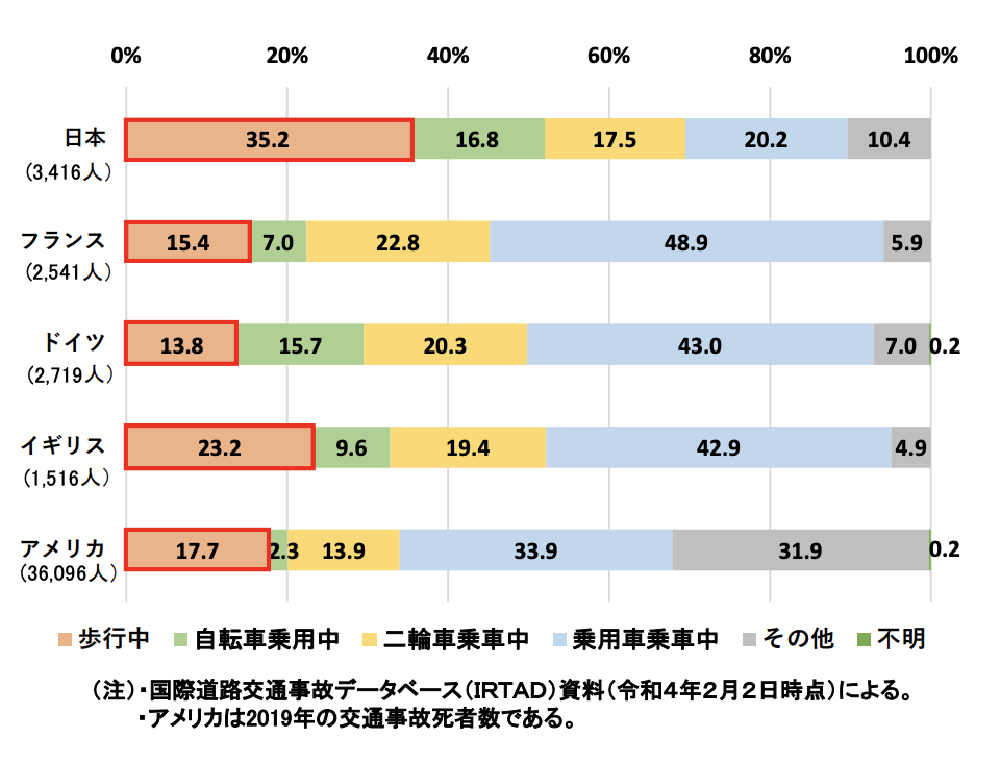
\includegraphics[height=50mm]{images/shibou_status.eps}
\caption{国別状態別30日以内死者数の構成率比較\cite{literature1}}
\label{国別状態別30日以内死者数の構成率比較}
\end{figure}

本研究では,富山県内において発生した人身事故と物損事故のデータを用いて特定の種類の事故がもつ特徴を分析することで,物損事故発生地点における人身事故の発生リスクの要因分析を行う.


\section{本研究で用いるデータ}
本研究では,富山県警から入手した平成29〜令和3年に富山県内で発生した人身事故データ(Fig.\ref{人身事故データ})と令和3年に発生した物損事故データ(Fig.\ref{物損事故データ})を用いる.
\begin{figure}[htb]
\centering
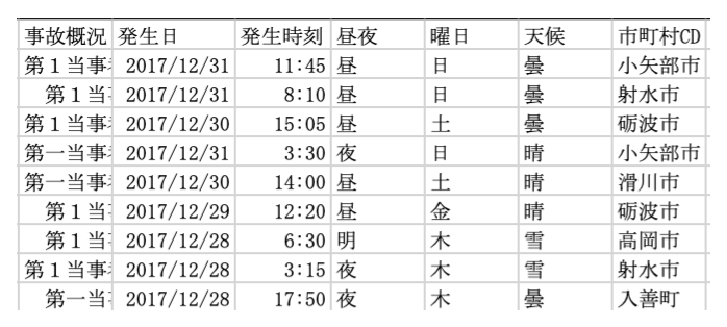
\includegraphics[height=30mm]{images/jinshixn.eps}
\caption{人身事故データ(一部抜粋)}
\label{人身事故データ}
\end{figure}

\begin{figure}[htb]
\centering
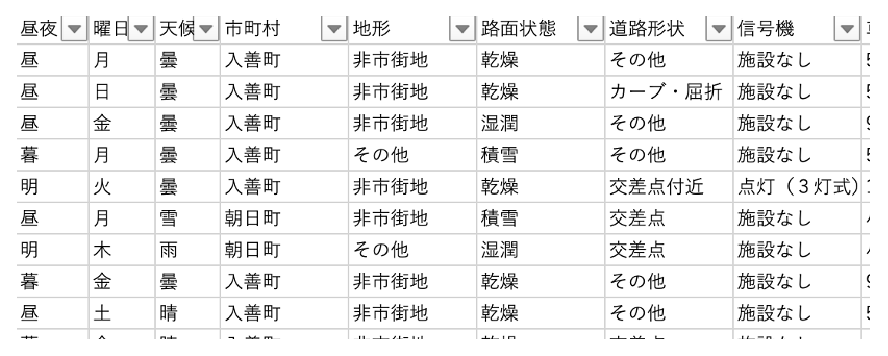
\includegraphics[height=30mm]{images/bussoxn.eps}
\caption{物損事故データ(一部抜粋)}
\label{物損事故データ}
\end{figure}

\section{本研究における分析手法}
\subsection{クラス分類}
線形サポートベクターマシン,非線形サポートベクターマシン,勾配ブースティングなど
のどれかを使う。図を用いて説明を入れる。

どれ使うかかんがえちゅう。
試しに簡単なクラスタ^ー分析を行った結果としては,勾配ブースティング決定木が一番いい感じだった

\subsection{形式概念分析}
形式概念分析 ( Formal Concept Analysis )は1981年のBanff 会議"Ordered Sets"においてRudolf Wille 氏によって提案されたデータ分析手法である\cite{literature2}.
形式概念分析を用いることで,共通の属性を持つオブジェクト集合と,その共通の属性集合の組み(コンセプト)を数学的に定義された概念データとして扱い,複雑なデータの構造の分析や,属性間に成り立つ含意論理の抽出によるデータ全体が持つ傾向分析を行うことが可能である。

本研究では,クラスター分析による要因


\section{クラス分類手法の選定}
\subsection{分類手法の選定}
本研究では分析手法として、クラス分類(Fig.\ref{classifications})を用いる。本研究で用いる分析手法の候補として、線形サポートベクターマシン、非線形サポートベクターマシン、勾配ブースティング決定枝が挙げられる。

\begin{figure}[htb]
\centering
\includegraphics[height=20mm]{images/no_image.eps}
\caption{線形サポートベクターマシンの例}
\label{classifications}
\end{figure}

\subsection{複数の分析手法によるクラスター分析の結果}
今のところ勾配ブースティング決定木が一番精度が良さそう

人身と物損両方を合わせて分析してみてから決める、でも大丈夫か?

\subsection{考察}
分析手法の選定が終わったら書くつもり

\section{分析用データ収集}
\subsection{物損事故、人身事故間のデータの差異}
(Fig.\ref{人身事故データ})と(Fig.\ref{物損事故データ})に示した、本研究で用いる人身事故データと物損事故データの間には、記録されている属性に違いがある。
本研究では分析にあたり、人身事故のみに保存されているデータの一部を物損事故に追加する手法を構築した。

\subsection{地図画像分類システム}
本研究では、道路線形や道路形状、信号の有無などを機械学習を用いて物損事故データに追加した。(Fig.\ref{地図画像分類システム})に簡易的なサーバ構成を示す。

本システムでは、Pythonで記述された画像分類アプリケーションがブラウザを介して物損事故発生地点周辺の地図画像を取得して、人身事故データを用いて学習した結果をもとに物損事故発生地点の情報を追加する。

なお、(Fig.\ref{地図画像分類システム})内"WebAPサーバ"は地図画像取得及び整形用スクリプトの配布サーバであり、Javaプラットフォーム向けのフレームワークであるSpringBoot\cite{literature3}を用いて作成した。また地図配布サーバはオープンソースソフトウェアであるmbtile-server\cite{literature4}を用いた。

\begin{figure}[htb]
\centering
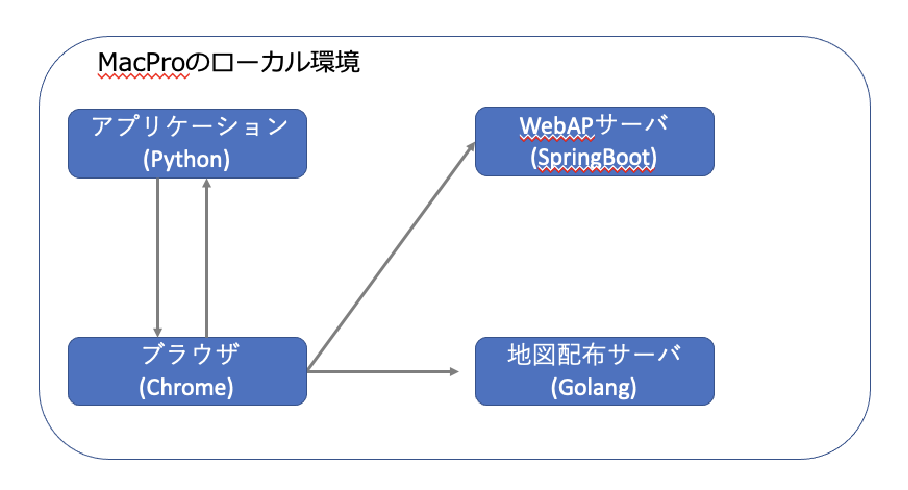
\includegraphics[height=30mm]{images/mapclassification_server.eps}
\caption{地図画像分類システム}
\label{classifications}
\end{figure}

\subsection{地図画像分類システムによるデータ追加の結果}
本システムを用いて地図画像分類を行った結果を図1に示す。

\section{考察}

\section{まとめ}
a

\begin{thebibliography}{9}
\bibitem{literature1}警察庁交通局,令和3年における交通事故の発生状況等について, 2022
\bibitem{literature2}鈴木治,室伏俊明,形式概念分析-入門・支援ソフト・応用-,日本知能情報ファジィ学会誌,Vol.19, No.2, pp.103-142, 2007
\bibitem{literature3}Spring Boot, [https://spring.io/projects/spring-boot]
\bibitem{literature4}consbio, mbtileserver, [https://github.com/consbio/mbtileserver]




     
\end{thebibliography}


\end{document}

